\section{Diagramas de Procesos}

\begin{BPMN}{MCD}{Creación de Requisitos para Documentación}{}
    \PCitem{Participantes}{\begin{itemize}
    		\item Docentes de la Academias	
    		\item Comité de Evaluación Curricular
    		\item Colegio de Profesores
    		\item Dirección General 
    \end{itemize}}
    \PCitem{Objetivo}{La elaboración o rediseño  de las Unidades de Aprendizaje, ya sea de forma individual o en paquetes, que pertenecen a un Plan de Estudios en un Programa Académico del IPN.}
    \PCitem{Interrelación con otros procesos}{
    \begin{itemize}
    	\item Entrada: Requisito de rediseñar o diseñar una nueva Unidad de Aprendizaje en un Plan de Estudios.
    	\item Salida: Tiras de Unidades de Aprendizaje en un Plan de Estudios.
	\end{itemize}
    }
    \PCitem{Entradas}{Plantillas de creación de Unidades de Aprendizaje}
    \PCitem{Consumidores}{Unidad Académica}
    \PCitem{Salidas}{Tiras de unidades de aprendizaje}
    \PCitem{Precondiciones}{Carga de resumen del Plan de Estudios}
    \PCitem{Postcondiciones}{Finalización del diseño o rediseño de un Programa Académico}
    \PCitem{Tipo}{Operativo}
\end{BPMN}
En la figura \hyperref[fig:MCD]{BPMN-02 Proceso para la creación de una Unidad de Aprendizaje}

\begin{figure}[H]
        \centering
        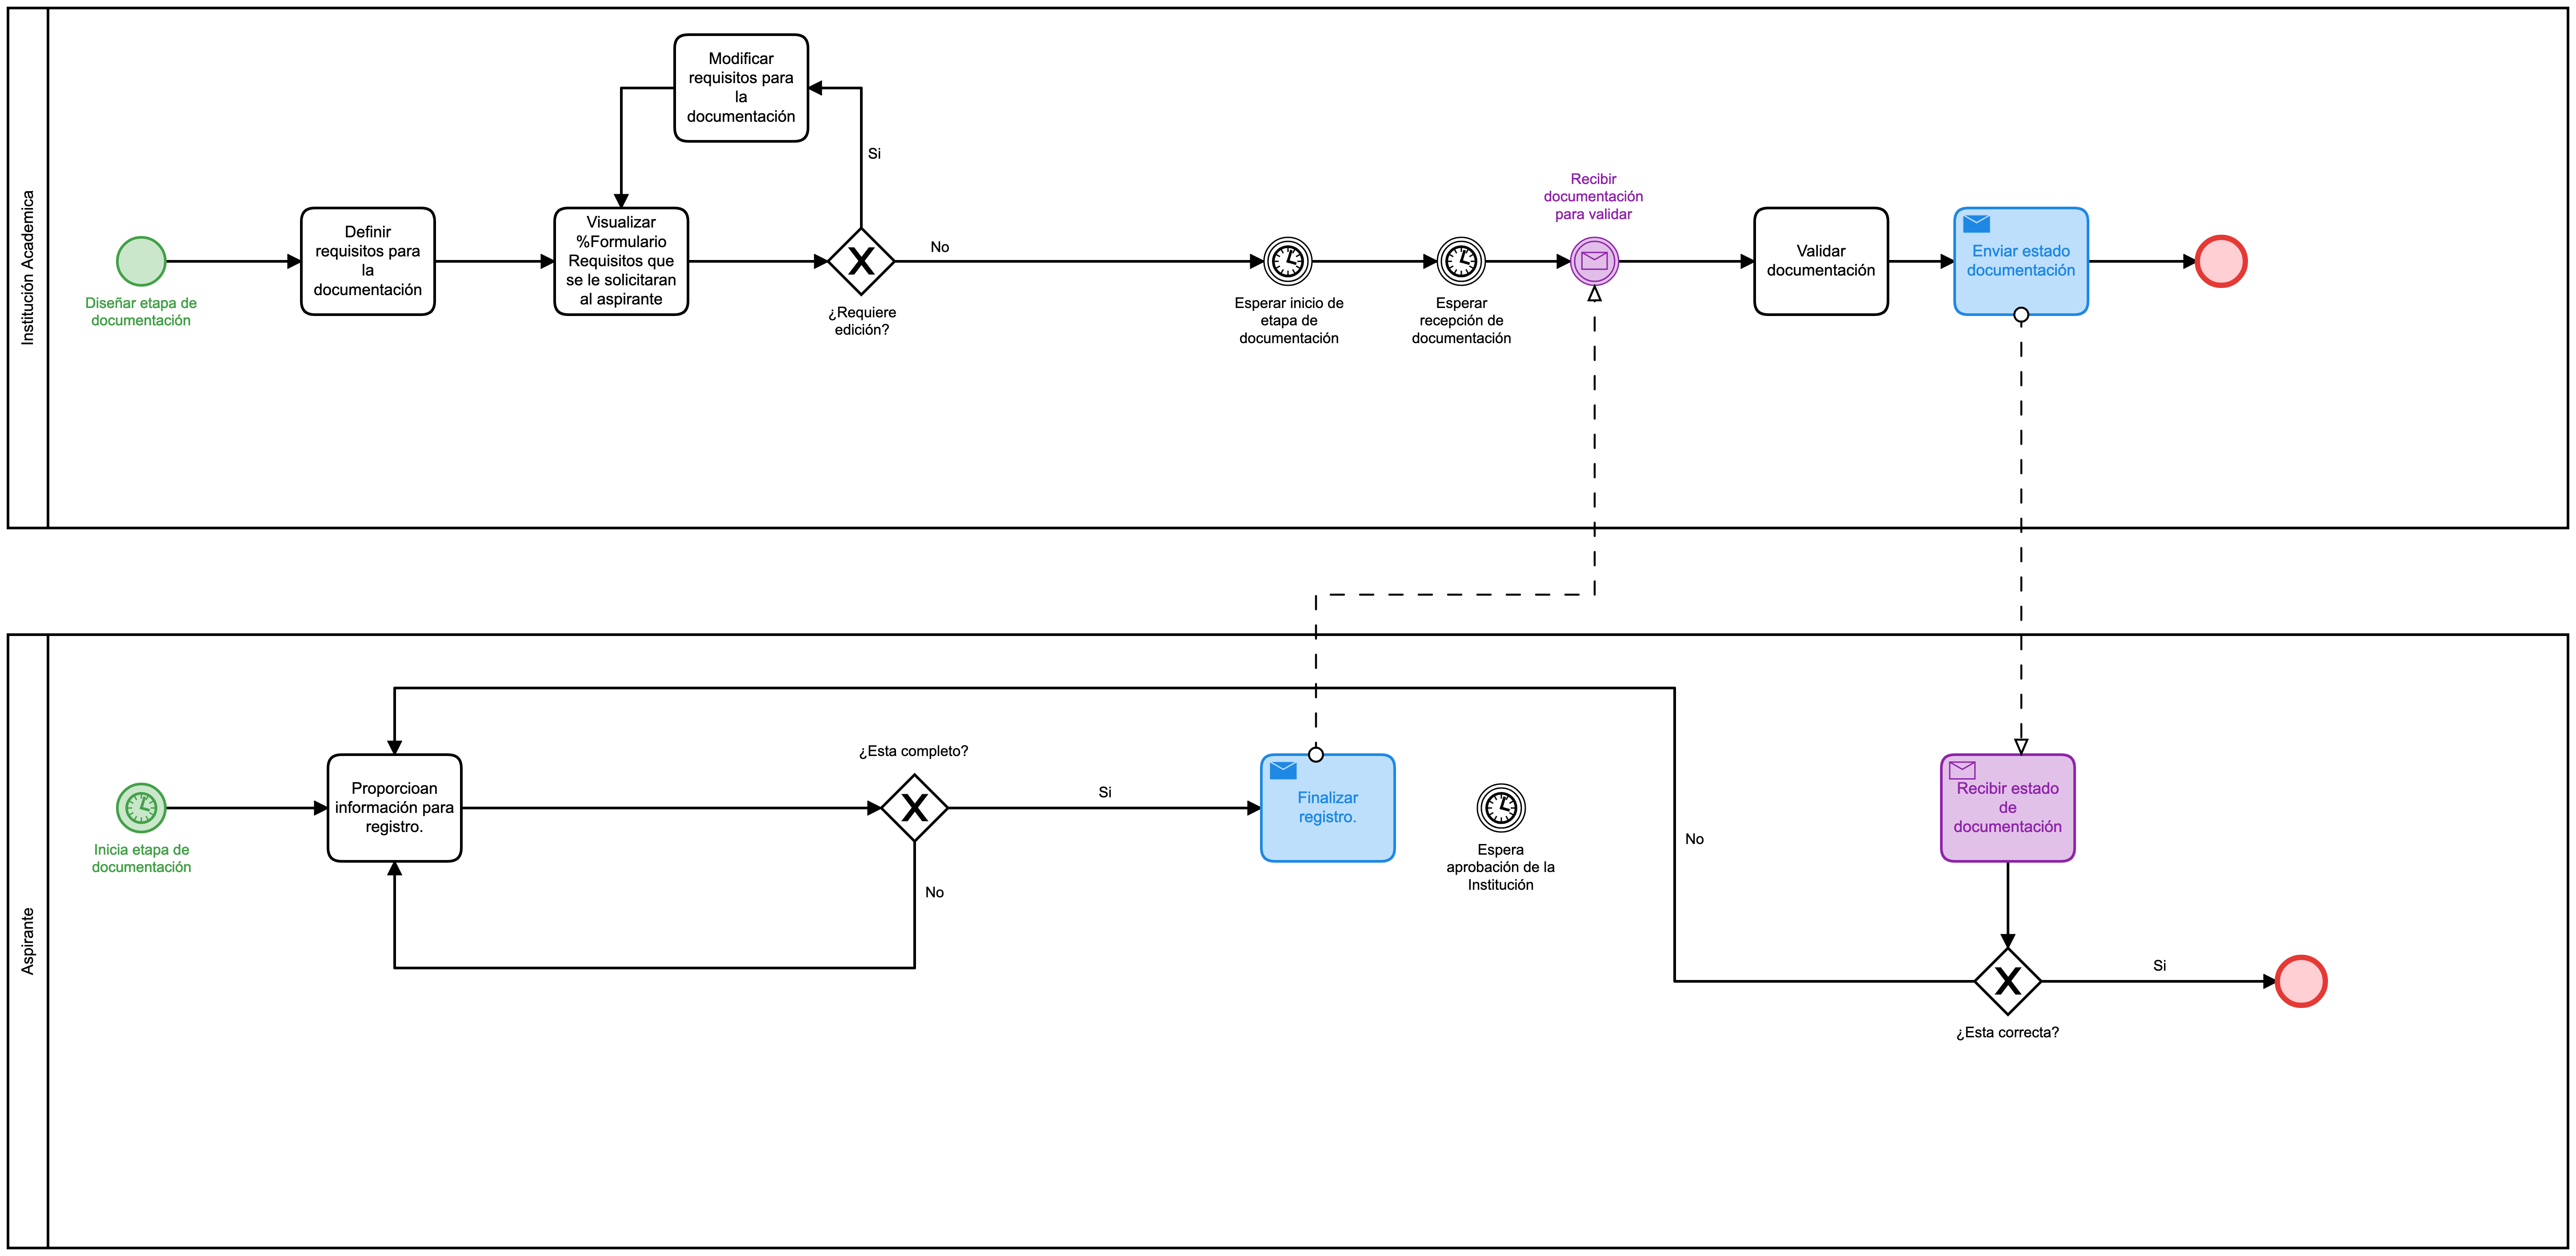
\includegraphics[width=1\textwidth]{TTI_2019-A055/imagenes/procesos/procesoDocumentacion.png}
        \caption{Proceso de Requisitos para Documentación.}
        \label{fig:MCD}
    \end{figure}
\newpage
\begin{itemize}
	\item \textbf{Elaborar instrumento para conocer el estado actual de la unidad de aprendizaje:} Se realiza la evaluación curricular dentro de la Unidad Académica para determinar la viabilidad de actualizar la Unidad de Aprendizaje.
	\item \textbf{Evaluación cuantitativa:}
	\item \textbf{Proporcionar instrumentos a los docentes:} Enviar los instrumentos y resultados de la evaluación curricular a los docentes encargados de la realización de la Unidad de Aprendizaje.
	\item \textbf{Elaborar informe:} Los docentes encargados, con base a los resultados obtenidos en la evaluación, realizan el informe del estado actual de la Unidad de Aprendizaje.
	\item \textbf{Elaborar diagnóstico:} Se determina si se aprueba o se rechazan los procesos de diseño o rediseño de la Unidad de Aprendizaje, según el informe del estado actual y la evaluación realizada.
	\item \textbf{Elaborar la "Descripción general de la Unidad de Aprendizaje":} Iniciar los procesos de rediseño o diseño de la Unidad de Aprendizaje. Se describe la asignatura.
	
	\item \textbf{Diseñar el programa de la asignatura:} Se inician los procesos de llenado de los programas sintéticos y en extenso de la Unidad de Aprendizaje.
	\item \textbf{Enviar a revisión:}  Los docentes envían los programas de la asignatura al Colegio de Profesores para su revisión.
	\item \textbf{Analizar el programa de la asignatura:} Se inician los trabajos de revisión de los programas sintéticos y en extenso de la Unidad de Aprendizaje por parte del Colegio de Profesores.
	
	\item \textbf{Enviar Unidad de Aprendizaje:}  Una vez aprobados los programas de la Unidad de Aprendizaje, se envían al Comité de Evaluación Curricular. Culmina el proceso.
	\item \textbf{Enviar ajustes:} Si existen correcciones o notas respecto a los programas de la Unidad de Aprendizaje, éstos se envían junto a ésta de vuelta a los docentes para ser atendidos.    
\end{itemize}

\pagebreak

% Procesos que yo debo de hacer
\begin{BPMN}{MGE}{Proceso del Modulo de Gestión de Etapas}{El proceso consiste en gestionar o bien configurar el orden de las etapas del proceso de admisión escolar las cuales son: convocatoria, recepción de documentos, pagos, evaluación y publicación de resultados, el único actor que interactúa en este proceso es el administrador root el cual tiene como tareas seleccionar las etapas que desee, ordenarlas, definir el periodo de cada una de las etapas y visualizarlas.}
    \PCitem{Participantes}{\begin{itemize}
    		\item Administrador Root.
    \end{itemize}}
    \PCitem{Objetivo}{Desarrollar una estrategia que permita configurar el orden de módulos para el sistema, para que se ajusten a la medida de cualquier institución.}
    \PCitem{Interrelación con otros procesos}{
    \begin{itemize}
    	\item Entrada: Iniciar Sesión.
    	\item Salida: El primer modulo de la etapa de proceso de admisión escolar que el administrador haya asignado..
	\end{itemize}
	}
    \PCitem{Entradas}{}
    \PCitem{Consumidores}{}
    \PCitem{Salidas}{Etapas configuradas.}
    \PCitem{Precondiciones}{El administrador root debe de iniciar sesión.}
    \PCitem{Postcondiciones}{Finalización de la seleción y orden de las etapas de proceso de admisión escolar.}
    \PCitem{Tipo}{Operativo}
\end{BPMN}
En la figura \hyperref[fig:MGE]{BPMN-02 Proceso para la creación de una Unidad de Aprendizaje}

\begin{figure}[H]
        \centering
        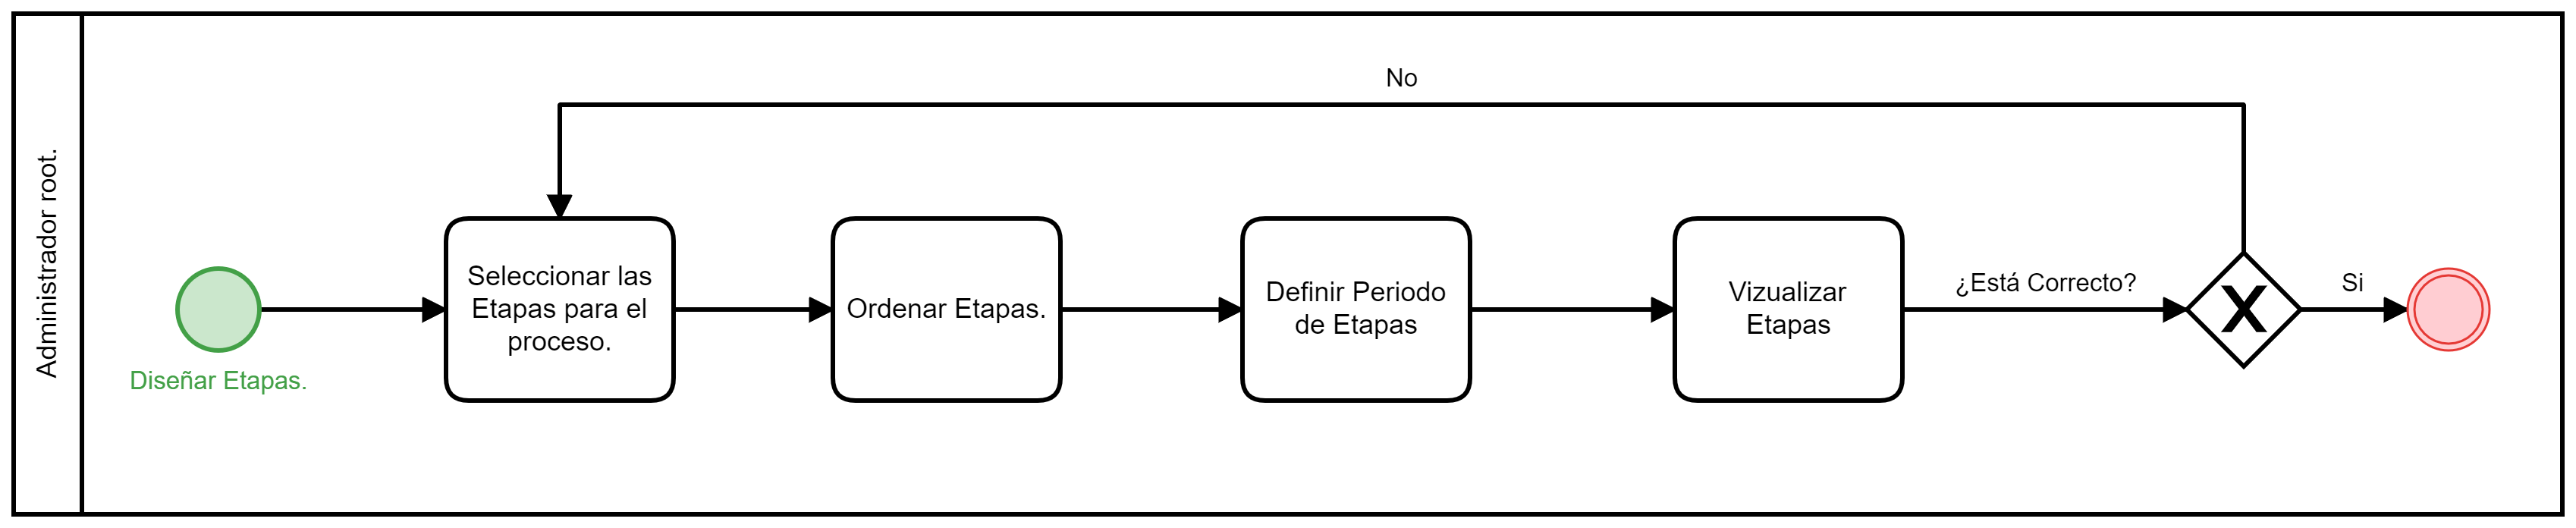
\includegraphics[width=1\textwidth]{TTI_2019-A055/imagenes/procesos/procesoGestionDeEtapas.png}
        \caption{Proceso de Gestión de Etapas.}
        \label{fig:MGE}
    \end{figure}

\begin{itemize}
	\item \textbf{Elaborar instrumento para conocer el estado actual de la unidad de aprendizaje:} Se realiza la evaluación curricular dentro de la Unidad Académica para determinar la viabilidad de actualizar la Unidad de Aprendizaje.
	\item \textbf{Evaluación cuantitativa:}
	\item \textbf{Proporcionar instrumentos a los docentes:} Enviar los instrumentos y resultados de la evaluación curricular a los docentes encargados de la realización de la Unidad de Aprendizaje.
	\item \textbf{Elaborar informe:} Los docentes encargados, con base a los resultados obtenidos en la evaluación, realizan el informe del estado actual de la Unidad de Aprendizaje.
	\item \textbf{Elaborar diagnóstico:} Se determina si se aprueba o se rechazan los procesos de diseño o rediseño de la Unidad de Aprendizaje, según el informe del estado actual y la evaluación realizada.
	\item \textbf{Elaborar la "Descripción general de la Unidad de Aprendizaje":} Iniciar los procesos de rediseño o diseño de la Unidad de Aprendizaje. Se describe la asignatura.
	
	\item \textbf{Diseñar el programa de la asignatura:} Se inician los procesos de llenado de los programas sintéticos y en extenso de la Unidad de Aprendizaje.
	\item \textbf{Enviar a revisión:}  Los docentes envían los programas de la asignatura al Colegio de Profesores para su revisión.
	\item \textbf{Analizar el programa de la asignatura:} Se inician los trabajos de revisión de los programas sintéticos y en extenso de la Unidad de Aprendizaje por parte del Colegio de Profesores.
	
	\item \textbf{Enviar Unidad de Aprendizaje:}  Una vez aprobados los programas de la Unidad de Aprendizaje, se envían al Comité de Evaluación Curricular. Culmina el proceso.
	\item \textbf{Enviar ajustes:} Si existen correcciones o notas respecto a los programas de la Unidad de Aprendizaje, éstos se envían junto a ésta de vuelta a los docentes para ser atendidos.    
\end{itemize}


    \begin{figure}[H]
        \centering
        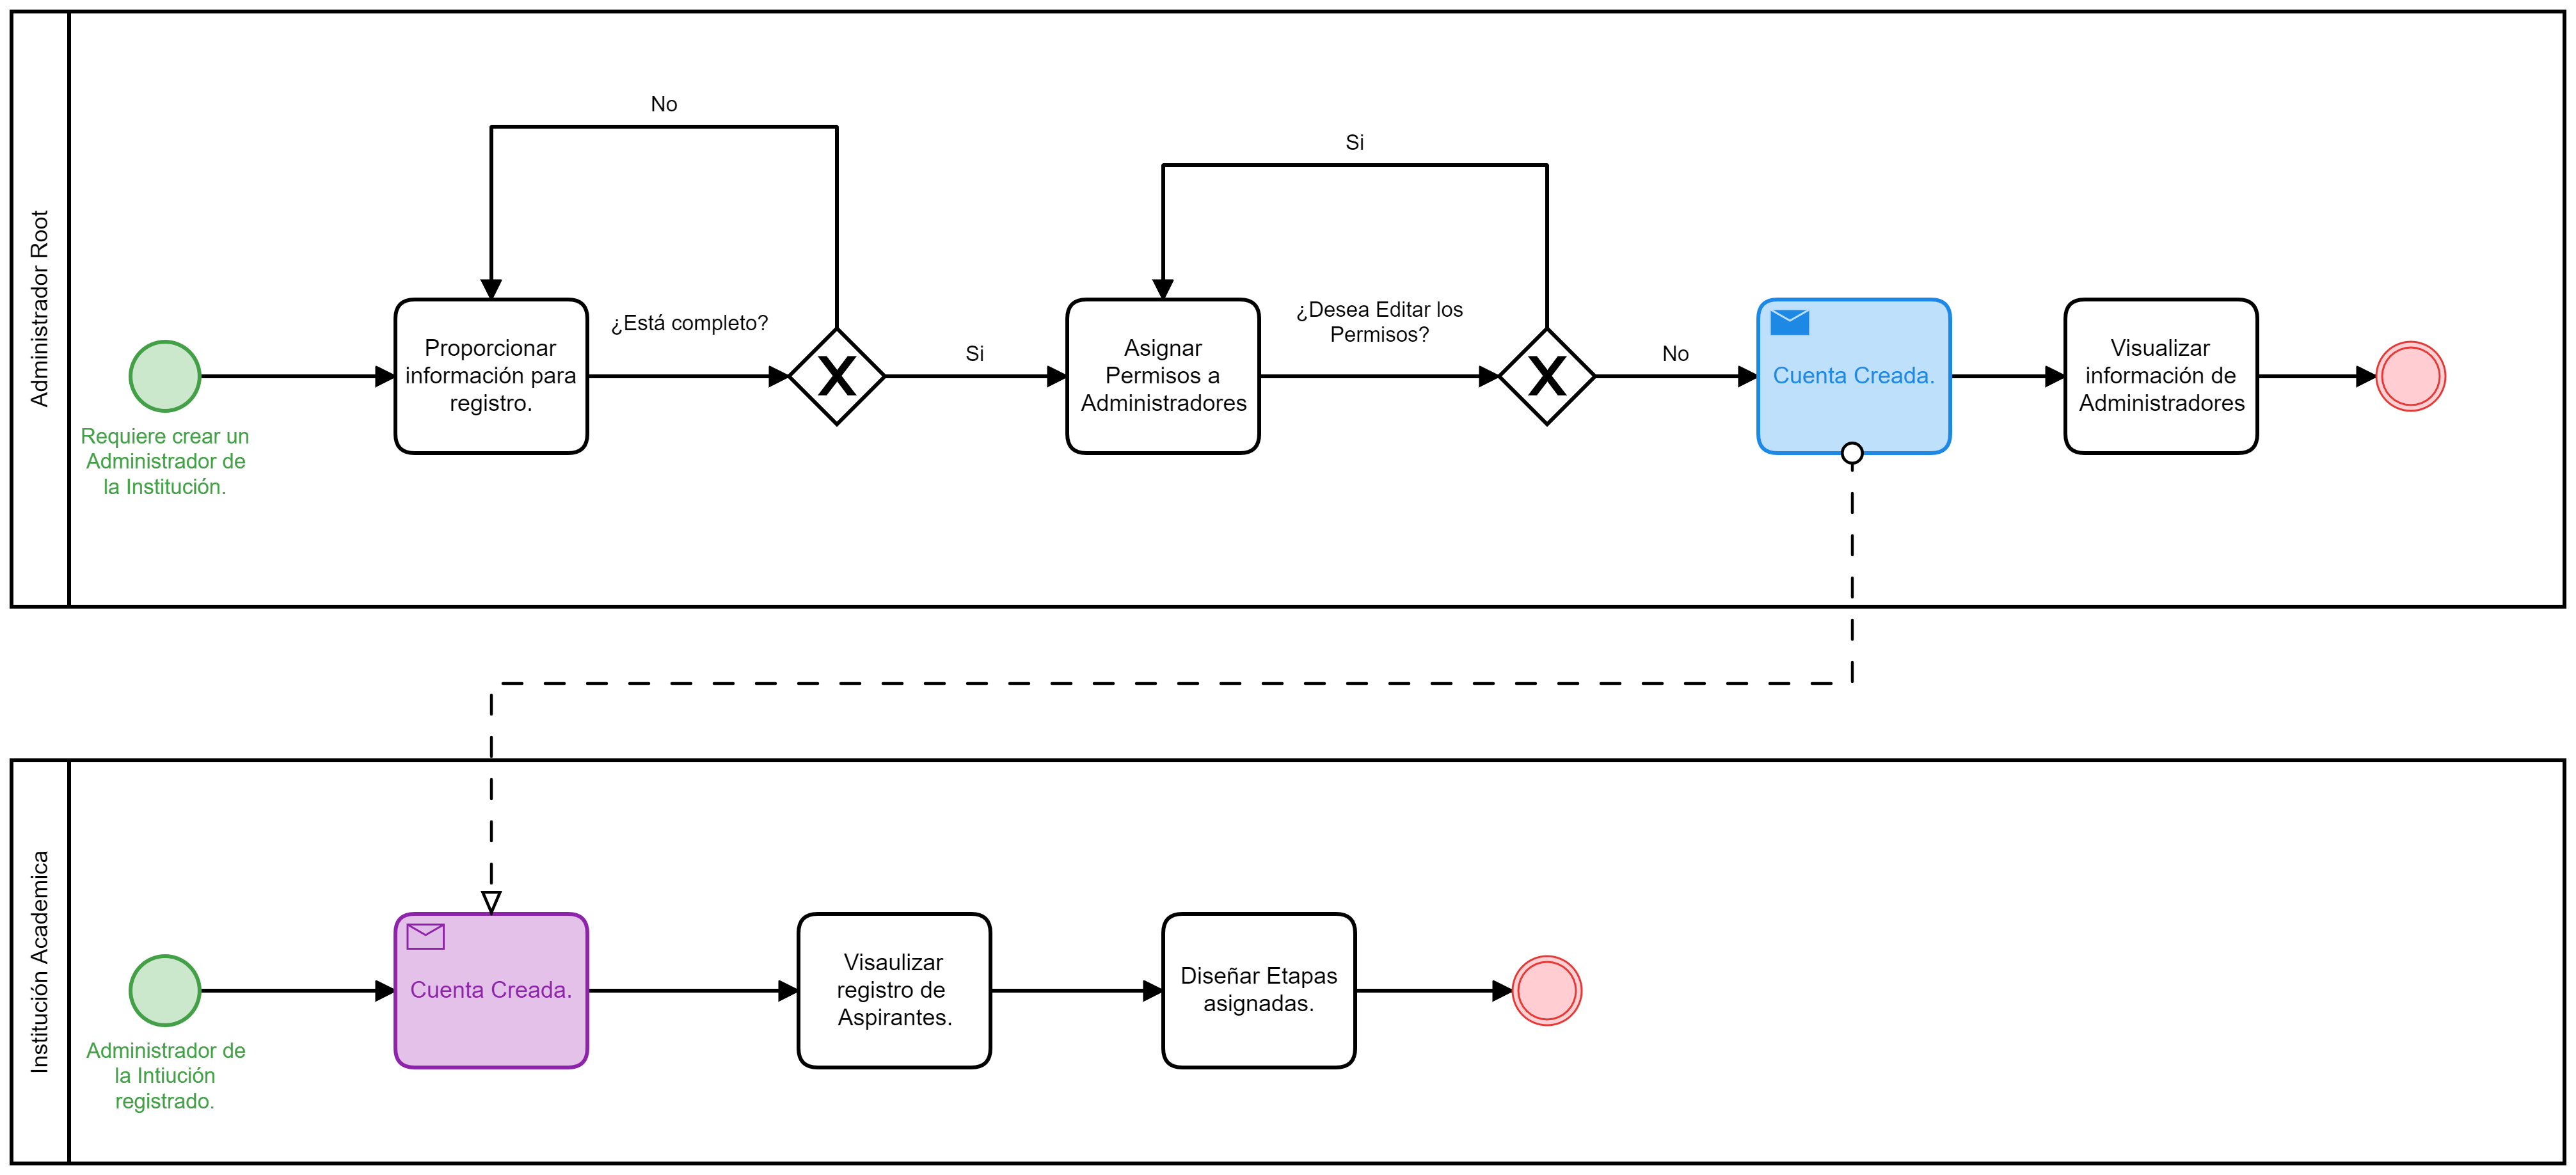
\includegraphics[width=1\textwidth]{TTI_2019-A055/imagenes/procesos/procesoGestionDeUsuarios.png}
        \caption{Proceso de Gestión de Usuarios.}
    \end{figure}
